\chapter{Introduction}
\section{Overview}
In today's interconnected digital landscape, the security of computer networks is of paramount
importance. With the increasing sophistication of cyber threats, organizations face a constant
challenge in safeguarding their networks from unauthorized access, malicious activities, and data
breaches. One crucial component of a comprehensive cybersecurity strategy is the Network
Intrusion Detection System (NIDS). A Network Intrusion Detection System (NIDS) is a vital
security tool designed to monitor network traffic in real-time, identifying and alerting administrators
to suspicious or potentially harmful activities. By analyzing network packets and patterns, NIDS
can detect various types of attacks, including malware infections, unauthorized access attempts,
denial-of-service (DoS) attacks, and more. This mini project report aims to explore the fundamentals
of Network Intrusion Detection Systems, including their functionalities, architecture, detection
techniques, and deployment strategies. Additionally, it will discuss the importance of NIDS in
enhancing network security posture, mitigating risks, and safeguarding critical assets against cyber
threats. Through this project, we seek to gain a deeper understanding of NIDS and its role in modern
cybersecurity practices, providing insights into its implementation, configuration, and effectiveness
in protecting network infrastructures from emerging threats.

\begin{figure}[ht]
    \centering
    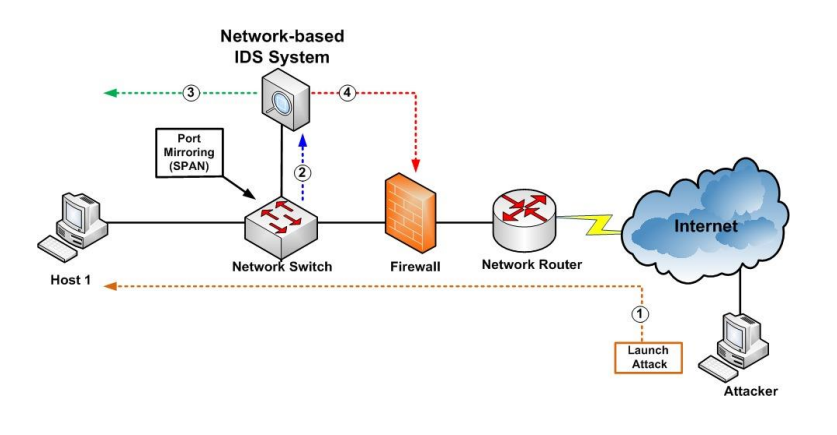
\includegraphics[width=0.8\textwidth]{images/nids.png}
    \caption{Network Intrusion Detection System.}
    \label{fig:single}
\end{figure}

The architecture of a typical NIDS consists of sensors strategically deployed throughout the
network infrastructure to capture and analyze traffic. These sensors can be hardware-based
appliances, software applications running on dedicated servers, or even virtual appliances
deployed in cloud environments. Central to the NIDS architecture is the analysis engine,
responsible for processing and correlating network data collected by the sensors, identifying
suspicious patterns, and generating alerts for further investigation. NIDS operates by
inspecting incoming and outgoing network traffic, comparing it against pre-defined signatures
or behavioral patterns indicative of known attacks or anomalies. Signature-based detection
involves matching network traffic against a database of predefined attack patterns or signatures,
allowing NIDS to recognize and respond to known threats effectively. On the other hand,
anomaly-based detection relies on establishing a baseline of normal network behavior and
flagging deviations from this baseline as potential intrusions. Additionally, some NIDS
solutions utilize a combination of signature-based and anomaly-based detection techniques for
enhanced accuracy and coverage.

\section{About the Project}
The "Network Intrusion Detection Using ML" project focuses on developing an advanced
intrusion detection system by harnessing machine learning (ML) algorithms and
methodologies. The primary goal is to design ML-based models capable of detecting and
mitigating various types of network intrusions, such as unauthorized access, malware
infections, data exfiltration, and insider threats. By training these models on labeled datasets
containing normal and malicious network traffic, the project aims to enhance network security
by leveraging ML's ability to identify sophisticated attacks that traditional methods may miss.
The initiative seeks to address the challenges posed by the evolving cyber threat landscape and
bolster the resilience of organizational networks against emerging security risks.

\section{Motivation}
The motivation behind the "Network Intrusion Detection Using ML" project is driven by the
exponential growth of cyber threats and attacks, which have posed significant challenges to the
security of computer networks. Traditional network intrusion detection systems (IDS) based on
rule-based approaches often struggle to keep pace with the ever-evolving attack landscape. This
necessitates the exploration of innovative solutions to enhance network security.

\subsection{Key Motivation}
\begin{itemize}
    \item \textbf{Limitations of Traditional IDS:}
    \begin{itemize}
        \item Rule-based IDS systems can be rigid and struggle to adapt to new, sophisticated attack vectors.
        \item Keeping up with the rapid evolution of cyber threats requires more flexible and adaptive approaches.
    \end{itemize}
    \item \textbf{Harnessing the Power of Machine Learning:}
    \begin{itemize}
        \item Machine learning techniques have demonstrated the ability to discern complex patterns and anomalies within large datasets.
        \item ML-based models can potentially identify sophisticated attacks that traditional methods may overlook.
    \end{itemize}
    \item \textbf{Enhancing Real-Time Threat Detection:}
    \begin{itemize}
        \item Timely detection and mitigation of network intrusions are crucial for maintaining the integrity and availability of organizational networks.
        \item Leveraging ML can enable real-time analysis and response to emerging security threats.
    \end{itemize}
    \item \textbf{Improving Network Resilience:}
    \begin{itemize}
        \item Strengthening network security is essential to ensure the resilience of critical infrastructure and safeguard sensitive data.
        \item Developing an advanced, ML-powered intrusion detection system can contribute to the overall security posture of organizations.
    \end{itemize}
\end{itemize}
    By harnessing the capabilities of machine learning, the \textit{Network Intrusion Detection Using ML} project aims to address the growing challenges in network security and bolster the resilience of organizational networks against evolving cyber threats.


\section{Challenges}
Based on the challenges outlined in the provided sources, here is a general arrangement based on their potential impact and prevalence:

\begin{enumerate}
    \item \textbf{Encrypted Traffic:} The increasing use of encryption protocols poses a significant challenge for intrusion detection systems as they struggle to inspect encrypted traffic effectively.
    \item \textbf{Zero-Day Attacks:} Zero-day attacks exploit unknown vulnerabilities without identifiable signatures, making them difficult to detect and defend against using traditional methods.
    \item \textbf{False Positives and Negatives:} Balancing detection sensitivity to minimize false alerts while accurately identifying malicious activity is crucial for the effectiveness of network intrusion detection systems.
    \item \textbf{Evasion Techniques:} Cyber attackers develop evasion techniques to bypass detection, necessitating continuous adaptation and improvement of detection mechanisms.
    \item \textbf{High Volume of Network Traffic:} Managing the large volume of network traffic and processing it in real-time without compromising detection accuracy is a fundamental challenge for intrusion detection systems.
    \item \textbf{Network Complexity:} The increasing complexity of network environments, including diverse assets and architectures, complicates the deployment and management of intrusion detection systems.
    \item \textbf{Resource Constraints:} Deploying intrusion detection systems in resource-constrained environments, like edge networks or IoT devices, presents challenges related to performance optimization and resource utilization.
    \item \textbf{Privacy Concerns:} Balancing effective intrusion detection with user privacy rights is essential to ensure that sensitive information is not compromised during monitoring and analysis.
\end{enumerate}

This arrangement highlights the diverse challenges faced in implementing machine learning for network security and underscores the importance of addressing these issues to enhance the effectiveness of intrusion detection systems.

\section{Problem Definition}
The "Network Intrusion Detection Using ML" project addresses the challenge of network
security amid increasing cyber threats. Traditional rule-based intrusion detection systems
struggle to keep pace with evolving attacks, prompting the exploration of advanced approaches.
By leveraging machine learning techniques, the project aims to develop an enhanced intrusion
detection system capable of identifying various network attacks in real-time. ML algorithms
analyze large datasets of network traffic to detect complex patterns and anomalies, improving
detection accuracy. This project is crucial as organizations rely more on interconnected
systems. Integrating ML into network security practices promises to strengthen defenses
against evolving threats, contributing to the security of critical network infrastructures.

\section{Aim}
The aim of the "Network Intrusion Detection Using ML" project is to develop an advanced
intrusion detection system that leverages machine learning techniques to effectively identify
and mitigate various types of network attacks in real-time, thereby enhancing the security and
resilience of organizational network infrastructures.

\section{Objectives}
\begin{enumerate}
    \item \textbf{Comprehensive Datasets:} IDSs should leverage up-to-date and comprehensive datasets for accurate evaluation, avoiding outdated or limited datasets that may lead to inaccurate results and false confidence in attack detection.
    \item \textbf{False Positive Reduction:} Efforts should be made to minimize false positives generated by IDSs, as a high false positive rate can lead to alert fatigue and hinder the ability of system administrators to respond effectively to actual attacks.
    \item \textbf{Zero-Day Attack Detection:} IDSs should incorporate advanced techniques, such as behavior-based anomaly detection and machine learning, to detect and respond to emerging and previously unseen attack patterns that do not have pre-defined signatures or rules.
    \item \textbf{Timely Detection and Response:} Improve IDSs for prompt identification and mitigation of network intrusions, addressing challenges like false positives and latency issues. Enhance algorithms, optimize data processing, and implement efficient detection mechanisms for timely threat response.
\end{enumerate}
